% !TEX program = xelatex
\documentclass{ctexart}

%\usepackage{CJKutf8}
% \usepackage{amsmath}
\usepackage[utf8]{inputenc}
\usepackage[a4paper,top=2cm,bottom=2cm,left=3cm,right=3cm,marginparwidth=1.75cm]{geometry}
\usepackage{tikz}
\usepackage{outlines}
\usepackage{amsthm}
\usepackage{mathtools}
\usepackage{xcolor}
\usepackage{graphicx}
\usepackage{float}
\usetikzlibrary{automata,positioning}
\newcommand{\hl}[1]{\colorbox{yellow}{#1}}
\newcommand{\tto}{\Rightarrow}
\graphicspath{ {./images/} }

\title{形式语言与自动机理论 笔记}
\author{Leo Lu}

\ctexset{
    section = {
        titleformat = \raggedright,
        name = {,},
        number = 第\chinese{section}章
    },
    paragraph = {
        runin = false
    },
    today = small,
    figurename = 图,
    contentsname = 目录,
    tablename = 表,
}

\newtheorem{definition}{定义}[section]
\newtheorem{example}{例}[section]
\DeclarePairedDelimiter{\set}{\{}{\}}
\DeclarePairedDelimiter{\paren}{(}{)}


\begin{document}
%\begin{CJK}{UTF8}{gbsn}

\maketitle

蒋宗礼\ 信息楼214\ jiangzl@bjut.edu.cn


\section{第一章 绪论}
\subsection{引入: 过河问题}
人 -> m 狼 -> w 羊 -> g 白菜 -> c
初状态: 
\begin{verbatim}
mwgc -
wc   - mg
mwc  - g
c    - mwg
mgc  - w
g    - mcw
mg   - cw
     - mgcw
\end{verbatim}
\subsection{重要性}
GRE中80道题,其中有8~15道形式语言。
\subsection {Basic Concepts}

\subsubsection{Alphabet}
An alphabet is a collection of characters.

Product of two alphabets:	
$$
\set*{0,1} \times \set*{a,b} = \set*{0a, 0b, 1a, 1b}
$$
Power of an alphabet:
$$
\Sigma^0 = {\epsilon}, \Sigma^n = \Sigma^{n-1} \times \Sigma
$$
Positive closure of an alphabet:
$$
\Sigma^+ = \bigcup_{i=1}^{\infty}\Sigma^i
$$
Kleene closure of an alphabet:
$$
\Sigma^* = \bigcup_{i=0}^{\infty}\Sigma^i = \set*{\epsilon} \cup \Sigma^+
$$

\subsubsection{Senctence}
X is a ``Sentence'' if:$\forall X \in \Sigma^*$

\subsubsection{Empty sentence}
An empty sentence, denoted by $\epsilon$ or $\lambda$, is a string with no characters at all.

\subsubsection{``Length'' of a ``Sentence''}

$\forall X \in \Sigma^*$, the count of characters appeared in x is called the length of x, denote by $\left|x\right|$

For example: $\left|ababab\right| = 6; \left|\epsilon\right| = 0$ 

\emph{Note that $\set*{\epsilon} \neq \Phi$}.

\subsubsection{Concatenation of sentences}
$\forall x, y \in \Sigma^*$, the concatenation of sentences $x, y$, denoted by $|xy|$, is the direct join of two strings.

$$
\left|xy\right| = |x| + |y|
$$

\subsubsection{N-power of sentences}
$\forall x \in \Sigma^*$, the n-power of sentence x:
$$
x^n = \begin{dcases*}
\epsilon & n=0 \\
x^{n-1}x & Other \\
\end{dcases*}
$$

\subsubsection{Prefix and Suffix}
$\forall x,y,z,w,v \in \Sigma^*$, given that $x=yz, w=yv$, then:
\begin{enumerate}
	\item $y$ is the Prefix of $x$
	\item $z$ is the Suffix of $x$
	\item if $z \neq \epsilon$, $y$ is "Proper Prefix" of $x$
	\item if $y \neq \epsilon$, $z$ is "Proper Suffix" of $x$
	\item $y$ is the "Common Suffix" of $x$ and $w$
\end{enumerate}
For example, if $x = 0110$:
\begin{itemize}
	\item Prefix of x is $\epsilon, 0, 01, 011, 0110$
	\item Proper prefix of x is $\epsilon, 0, 01, 011$
	\item Suffix of x is $\epsilon, 0, 10, 110, 0110$
	\item Proper suffix of x is $\epsilon, 0, 10, 110$
\end{itemize}

\subsubsection{Reverse of a sentence}

	The reverse of sentence $x$ is denoted by $x^R$ or $x^T$.

\subsubsection{Language on Alphabet $\Sigma$}

	$\forall L \subseteq \Sigma^*$, $L$ is called {a Language on alphabet $\Sigma$} \par
	$\forall x \in L$, $x$ is called \emph{a sentence of $L$}

	For example: let $\Sigma = \set*{0, 1}$, we have
	\begin{enumerate}
		\item $L_1 = \set*{0, 1}$
		\item $L_2 = \set*{00, 01, 10, 11}$
		\item $L_3 = \set*{0, 1, 00, 01, 10, 11, \dots } = \Sigma^+$
		\item $L_4 = \set*{\epsilon, 0, 1, 00, 01, 10, 11, \dots} = \Sigma^*$
		\item $L_5 = \set*{0^n | n \ge 1}$
		\item $L_6 = \set*{0^n1^n | n \ge 1 }$
		\item $L_7 = \set*{1^n | n \ge 1 }$
		\item $L_8 = \set*{0^n1^m | n, m \ge 1 }$
		\item $L_9 = \set*{0^n1^n0^n | n \ge 1 }$
		\item $L_{10} = \set*{0^n1^m0^k | n,m,l \ge 1}$
		\item $L_{11} = \set*{x | x \in \Sigma^+ \text{and the number of 0 and 1 of x are same}}$
	\end{enumerate}

\subsubsection{Operation of Language}

All operatio on Sets also works on Language.

\emph{Note that $\cup, \cap, -, \overline{\ }$ are closure(封闭的)}.

\textbf{Product of Languages:}

Given $L_1 \subseteq \Sigma_1^*, L_2 \subseteq \Sigma_2^*$, the product of $L_1$ and $L_2$ is a Language on alphabet $\Sigma_1 \cup \Sigma_2$.

$$
L_1L_2 = \set*{xy | x \in L_1, y \in L_2 }
$$


\textbf{Power of Languages}:

Given a language $L$, we have:
$$
L^n = \begin{cases}
\epsilon & n=0 \\
L^{n-1}L & Other \\
\end{cases}
$$

\textbf{Positive closure of a language:}
$$
L^+ = \bigcup_{i=1}^{\infty}L^i
$$

\textbf{Kleene closure of a language:}
$$
L^* = \bigcup_{i=0}^{\infty}L^i = \set*{\epsilon} \cup L^+
$$

Note that: $L^+ = L^* \iff \epsilon \in L$

% \begin{tikzpicture}[shorten >=1pt,node distance=2cm,on grid,auto] 
%    \node[state,initial] (q_0)   {$q_0$}; 
%    \node[state] (q_1) [above right=of q_0] {$q_1$}; 
%    \node[state] (q_2) [below right=of q_0] {$q_2$}; 
%    \node[state,accepting](q_3) [below right=of q_1] {$q_3$};
%     \path[->] 
%     (q_0) edge  node {0} (q_1)
%           edge  node [swap] {1} (q_2)
%     (q_1) edge  node  {1} (q_3)
%           edge [loop above] node {0} ()
%     (q_2) edge  node [swap] {0} (q_3) 
%           edge [loop below] node {1} ();
% \end{tikzpicture}

\textbf{Examples}
\begin{outline}
    \1 给定 $\Sigma$, 讨论$\Sigma$上典型语言的结构特征
        \2 $\set*{0^n1^m | n, m \geq 1}$:
        \begin{center}
            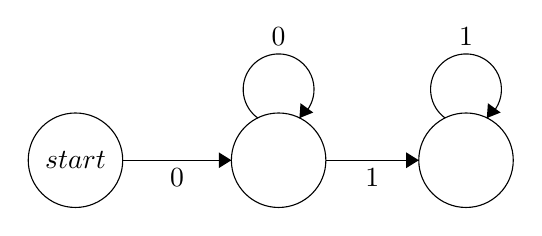
\begin{tikzpicture}[scale=0.2]
            \tikzstyle{every node}+=[inner sep=0pt]
            \draw [black] (9.1,-16.3) circle (3);
            \draw (9.1,-16.3) node {$start$};
            \draw [black] (22,-16.3) circle (3);
            \draw [black] (33.9,-16.3) circle (3);
            \draw [black] (12.1,-16.3) -- (19,-16.3);
            \fill [black] (19,-16.3) -- (18.2,-15.8) -- (18.2,-16.8);
            \draw (15.55,-16.8) node [below] {$0$};
            \draw [black] (20.677,-13.62) arc (234:-54:2.25);
            \draw (22,-9.05) node [above] {$0$};
            \fill [black] (23.32,-13.62) -- (24.2,-13.27) -- (23.39,-12.68);
            \draw [black] (25,-16.3) -- (30.9,-16.3);
            \fill [black] (30.9,-16.3) -- (30.1,-15.8) -- (30.1,-16.8);
            \draw (27.95,-16.8) node [below] {$1$};
            \draw [black] (32.577,-13.62) arc (234:-54:2.25);
            \draw (33.9,-9.05) node [above] {$1$};
            \fill [black] (35.22,-13.62) -- (36.1,-13.27) -- (35.29,-12.68);
            \end{tikzpicture}
            \end{center}
        \2 $\set*{0^n1^n0^n | n \geq 1}$
    \1 给定$\Sigma$, 讨论语言的结构与表示
        \2 $\set*{xx|x \in \Sigma^+\} = \{a_1a_2\dots a_na_1a_2 \dots a_n|a_1,a_2,\dots,a_n \in \Sigma, n \geq 1}$
        \2 $\set*{xx^T | x \in \Sigma^+}$
        \2 $\set*{xx^Tw | x,w \in \Sigma^+} \\ 
            = \set*{a_1a_2\dots a_n \dots a_1 b_1 \dots b_m | a_1,\dots, a_n, b_1, \dots, b_m \in \Sigma, n,m \geq 1}$
        \2 $\set*{xwx^T|x, w \in \Sigma^+}  \\ 
            = \set*{a_1 \dots a_n b_1 b_2 \dots b_n a_n \dots a_1 | a_1,\dots,a_n,b_1,\dots,b_m \in \Sigma, n,m \geq 1} \\
            = \set*{a a_1 \dots a_n a | a, a_1, a_2, \dots, a_n \in \Sigma, n \geq 1}
            $
\end{outline}

\section{第二章\ 文法} 
\subsection{启示}
\begin{outline}
    \1 对无穷对象的描述
        \2 $\set*{0^n | n \geq 1}$
            \3 $0$ 是 $S$的元素
            \3 $\forall x \in S, x0 \in S$
            \3 $S \to 0$
            \3 $S \to S0$
        \2 $\set*{0^n1^m | n, m \geq 1}$
            \3 $0 \in S$ \\
               $\forall x \in S, 0x, x1 \in S$
            \3 $S \to 01$ \\
               $S \to 0S | S1$
            \3 $S \to S_1S_2$ \\
               $S_1 \to 0$ \\
               $S_1 \to S_10$ \\
               $S_2 \to 0$ \\
               $S_2 \to S_20$
        \2 $\set*{0,1}^*$
            \3 $\epsilon \in S$ \\
               $\forall x \in S, 0x, 1x \in S$
            \3 $S \to \epsilon$ \\
               $S \to 0S $\\
               $S \to 1S $
        \2 $\set*{0,1\}^*\set*{11}\{0,1}^*$
            \3 $11 \in S$ \\
               $\forall x \in S, 0x, 1x, x0, x1 \in S$
            \3 $S \to 11$ \\
               $S \to 0S | 1S | S0 | S1$
    \1 如何定义中缀表达式:递归
        \2 描述:
            \3 $ident$是表达式
            \3 表达式加表达式是表达式
            \3 表达式减表达式是表达式
            \3 表达式乘表达式是表达式
            \3 表达式除表达式是表达式
            \3 表达式加括号是表达式
        \2 定义:
            \3 表达式\emph{定义为}标识符
            \3 表达式\emph{定义为}表达式$+$表达式
            \3 表达式\emph{定义为}表达式$-$表达式
            \3 表达式\emph{定义为}表达式$\times$表达式
            \3 表达式\emph{定义为}表达式$\div$表达式
            \3 表达式\emph{定义为}(表达式)
        \2 符号化 \par
               $E \to ident$ \\
               $E \to E + E$ \\
               $E \to E - E$ \\
               $E \to E \times E$ \\
               $E \to E \div E$ \\
               $E \to (E)$
        \2 表示优先级
            \3 因子是标识符
            \3 因子是括号的表达式
            \3 项是因子
            \3 项是因子$*/$因子
            \3 表达式是项
            \3 表达式是表达式$+-$表达式
        \2 符号化 
            \3 Variables: $E, T, F$
            \3 Terminals: $+ - \times \div ident ( )$
            \3 Products:  \\
                $E \to T + T$ \\
                $E \to T - T$ \\
                $E \to T$ \\
                $T \to F \times F$ \\
                $T \to F \div F$ \\
                $T \to F $ \\
                $F \to ident$ \\
                $F \to (E)$
            \3 Start Symbol: $E$
\end{outline}
\subsection{形式定义}
\begin{definition}
    文法(Grammar)G是一个四元组
    $$
        G = (V, T, P, S)
    $$
    其中,

    V--- \emph{变量(Variable)}的非空有穷集。$\forall A \in V$,
    $A$叫做语法变量(syntactic variable),也叫非终极符号(nonterminal)。
    
    T--- \emph{终极符(Terminal)}的非空有穷集。$\forall a \in T$,
    $a$叫做终极符。 $V \cup T = \Phi$。

    P--- \emph{产生式(Production)}的非空有穷集。对于$a \to b$,
    $a$是\emph{左部},$b$是\emph{右部}。

    S--- $S \in V$,文法G的\emph{开始符号(Start symbol)}。
\end{definition}

约定:
\begin{outline}
    \1 只写产生式,第一个产生式的左部为开始符号
    \1 对一组有相同左部的产生式 \\
        $\alpha \to \beta_1, \alpha \to \beta_2, \alpha \to \beta_3, \dots$
        可以记为 $\alpha \to \beta_1 | \beta_2 | \beta_3 \dots$
        $\beta_1 , \beta_2 , \beta_3$称为\emph{候选式}(Candidate)
    \1 形如$\alpha \to \epsilon$的产生式叫做空产生式,也可叫做$\epsilon$产生式
    \1 符号
        \2 英文大写字母为\emph{语法变量}
        \2 英文小写字母为\emph{终结符号}
        \2 英文较后的大写字母为\emph{语法变量或者终极符号}
        \2 英文较后的大写字母为\emph{终极符号行}
        \2 希腊字母表示\emph{语法变量和终极符号组成的行}
\end{outline}

\begin{definition}
    设$G = (V,T,P,S)$是一个文法,如果
    $\alpha \to \beta\in P, \gamma,\delta  \in (V \cup T)$,则称
    $\gamma\alpha\delta$在$G$中\emph{直接推导}(Derivation)出$\gamma\beta\delta$,记作
    $\gamma\alpha\delta \underset{G} \Rightarrow \gamma\beta\delta$。

    于此相对应,$\gamma\beta\delta$归约到$\gamma\alpha\delta$,简称$\beta$归约为$\alpha$。

    $\underset{G} \Rightarrow$ 是$\left( V \cup T \right)^*$上的二元关系。
\end{definition}

\begin{definition}对于文法$G$:

    $\underset{G}{\overset{n}\Longrightarrow } = \left(\underset{G} \Rightarrow \right)^n $ 

    $\underset{G}{\overset{*}\Longrightarrow } = \left(\underset{G} \Rightarrow \right)^* $

    $\underset{G}{\overset{=}\Longrightarrow } = \left(\underset{G} \Rightarrow \right)^+ $

    当只有唯一的文法$G$时,可以省略$G$:$\overset{n}\Longrightarrow, \overset{*}\Longrightarrow, \overset{+}\Longrightarrow$

\end{definition}

\begin{definition}
    对于语言$G = (V, T, P, S)$:

    语法范畴A $L(A) = \set*{w | w \in T^* \text{且} A \overset{*}\Rightarrow w}$

    语言(Language) $L(G) = \set*{w | w \in T^* \text{且} S \overset{*}\Rightarrow w}$

    句子(Sentence) $\forall w \in L(G)$

    句型(Sentential Form) $\forall \alpha \in (V \cup T)^*$, 
    如果$S \overset{*}\Rightarrow \alpha$,则称$\alpha$是$G$产生的一个句型。
    
\end{definition}

\begin{definition}
    对于文法 $G_1, G_2$,如果$L(G_1) = L(G_2)$,则称$G_1$与$G_2$等价。
\end{definition}

\subsection{文法的构造}
\begin{outline}
    \1 $L(G) = \set*{0,1,00,11}$
        \2 $G_1: S \to 0 | 1 | 00 | 11$
        \2 $G_2: S \to A | B | AA | BB, A \to 0, B \to 1$
        \2 $G_3: S \to 0 | 1 | 0A | 1B, A \to 0, B \to 1$
        \2 $G_4: S \to A | B | AA | BB, A \to 0, B \to 1, C \to 1$
    \1 $\set*{x | x \text{是至少3个1的0,1串}}$
        \2 $G: S \to A1A1A1A, A \to \epsilon| 0A| 1A$
        \2 $G: S \to A1A1A1B, A \to \epsilon | 0A, B \to \epsilon | 0B | 1B$
        \2 $G: S \to AAAB, A \to 1 | 0A, B \to \epsilon | 0B | 1B$
\end{outline}

\subsection{文法的乔姆斯体系}
\begin{definition}
    对于文法$G = (V,T,P,S)$: \\
    G叫做0型文法,Type 0 Grammar,也叫短语结构文法(PSG,Phrase Structure Grammar) \\
    $L(G)$是0型语言,也叫短结构语言,可递归枚举集。
\end{definition}
\begin{definition}
    对于0型文法文法$G = (V,T,P,S)$: \\
    如果对于$\forall \alpha \to \beta \in P$,均有$|\beta| \geq |\alpha|$,
    则G是1型文法,或上下文有关文法。
\end{definition}
\begin{definition}
    对于1型文法文法$G = (V,T,P,S)$: \\
    如果对于$\forall \alpha \to \beta \in P$,均有$|\beta| \geq |\alpha|$,
    并且$\alpha \in V$
    则G是2型文法,或上下文无关文法。
\end{definition}
\begin{definition}
    对于2型文法文法$G = (V,T,P,S)$: \\
    如果对于$\forall \alpha \to \beta \in P$: \\
    如果形如$A \to wB$和$A \to w$,其中$A,B \in V, w \in T^+$:G是右线性文法。 \\
    如果形如$A \to Bw$和$A \to w$,其中$A,B \in V, w \in T^+$:G是左线性文法。 \\
    则G是3型文法,或正则文法。
\end{definition}

\subsection{空产生式}
允许在CSG,CFG,RG文法中存在空产生式。 

允许在CSL,CFL,RL语言中存在空语句。

特点:
\begin{outline}
    \1 对于$\forall$右线性文法$G_1$,$\exists$ 左线性文法 $G_2$ 使得 
    $L(G_1) = L(G_2)$
    \1 对于$\forall$左线性文法$G_1$,$\exists$ 右线性文法 $G_2$ 使得 
    $L(G_1) = L(G_2)$ \\
        所以,某种意义上二者等价。其中,\emph{左线性文法的表述好。}\\
        \hl{\emph{左递归}?}
        \emph{线性文法不是正则文法!}
    \1 $\forall G, \exists G', L(G') = L(G)$,但是$G'$中的开好似符号不出现在任何
    产生式的右部,且在$\epsilon \in L(G')$时,$G'$中只有$S' \to \epsilon$这样一个
    $\epsilon$产生式。
\end{outline}

\subsubsection{语言运算}
给定上下文无关文法$G_1,G_2$,构造$G$使得:
\begin{outline}[enumerate]
    \1 $L(G) = L(G_1)L(G_2)$ \\
        其中$V_1 \cup V_2 = \phi$, $S \notin V_1 \cup V_2$

        $G = (V_1 \cup V_2 \cup {S}, T, P_1 \cup P_2 \cup {S \to S_1S_2}, S)$

    \1 $L(G) = L(G_1) \cup L(G_2)$

        $G_\cup = (V_1 \cup V_2 \cup {S}, T, P_1 \cup P_2 \cup P_3, S)$ \\
        $P_3 = \set*{S \to S_1 | S_2}$

    \1 $L(G) = L(G_1)^*$

        $G_* = \paren*{V_1 \cup \set*{S}, T, P_1 \cup P_2, S}$ \\
        $P_2 = \set*{S \to \epsilon | SS_1}$

\end{outline}

给定RG $G_1,G_2$,构造RG $G$使得:
\begin{outline}[enumerate]
    \1 $L(G) = L(G_1)L(G_2)$ \\
        其中$V_1 \cup V_2 = \phi$, $S \notin V_1 \cup V_2$

        $\begin{aligned}
            S_1  & \tto a_1A_1 \\
                 & \tto a_1a_2\dots a_{n-1}A_n  \\
                 & \tto a_1a_2\dots a_nS_2
        \end{aligned}$
        所以,我们需要改造$P_1$。

        $G = (V_1 \cup V_2 \cup {S}, T, P_1' \cup P_2 \cup P_3, S_1)$

        $P_1' = \set*{A \to a B | A \to a B \in P_1}$
        
        $P_3 = \set*{A \to a S_2 | A \to a \in P_1}$

    \1 $L(G) = L(G_1) \cup L(G_2)$

        $G_\cup = (V_1 \cup V_2 \cup {S}, T, P_1 \cup P_2 \cup P, S)$ \\
        $\begin{aligned}
            P & = \set*{S \to \alpha | S_1 \to \alpha \in P_1} \\
            & \cup \set*{S \to \alpha | S_2 \to \alpha \in P_2} \\
        \end{aligned}$

    \1 $L(G) = L(G_1)^*$

        \hl{自己想!}
\end{outline}

例子:

\begin{outline}[enumerate]
    \1 设$L = \set*{x | 101 \text{ in } x}$,构造 $G, L(G) = L$。

    朴素构造:$\begin{cases}
        S \to A 101 A \\
        A \to \epsilon | 0A | 1A
    \end{cases}$
    
    正则构造:$\begin{cases}
        S \to 0S | 1A \\
        A \to 0B | 1A \\
        B \to 1C | 0S \\
        C \to 0C | 1C | \epsilon
    \end{cases}$

    \1 构造$G$使$L(G) = \set*{x | 101 \text{ not in } x}$

    正则构造:$\begin{cases}
        S \to 0S | 1A \\
        A \to 0B | 1A \\
        B \to 0S | \epsilon\\
    \end{cases}$
\end{outline}



\subsection{小结}


习题: p67 3,4,8.2,8.6,10.3,11.3

\section{有穷状态自动机 Finite Automata}

\subsection{FA的基本定义}
\begin{figure}[H]
    \centering
    \caption{有穷状态自动机}
    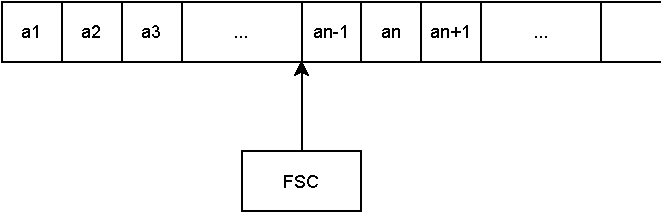
\includegraphics{FA}
\end{figure}

\begin{definition}
    $M = (Q, \Sigma, \delta, q_0, F)$,其中:

    \begin{description}
        \item[$Q$]:状态的有穷集合
        \item[$\Sigma$]: 输入字母表
        \item[$\delta$]: 状态转义函数\\
            $Q\times\Sigma \to Q$。 $\forall (q,a) \in Q\times\Sigma$,
            $\delta(q,a) = p$表示$M$在状态$q$读入一个字符$a$,状态改为$p$并
            指向下一个字符。
        \item[$q_0$]:开始状态
        \item[$F$]: 终止状态 
    \end{description}
\end{definition}
\begin{definition}
    有穷状态自动机$M = (Q, \Sigma, \delta, q_0, F)$:

    状态转移图是满足如下条件的有向图。
    \begin{enumerate}
        \item 对于$q \in Q$, $q$是一个顶点
        \item $\forall (q,a) \in \delta$, $q$到$p$有一条标记为$a$的弧。
        \item 标有S的箭头所指的状态为开始状态。
        \item 用双圈标记结束状态。
    \end{enumerate}

    扩展$\delta$为$\hat{\delta}: Q \times \Sigma^* \to Q$
    \begin{enumerate}
        \item $\hat{\delta}(q,\epsilon) = q$
        \item $\hat{\delta}(q, wa) = \delta(\hat{\delta}(q,w), a)$
    \end{enumerate}
    注意到 $Q \time \Sigma \subset Q \times \Sigma^*$,
    且对$\forall (q, a) \in Q \times \Sigma^*$,$\hat{\delta}(q, a) = \delta(q, a)$
    所以,不用区分$\delta$与$\hat{\delta}$
\end{definition}

\begin{definition}
    有穷状态自动机$M = (Q, \Sigma, \delta, q_0, F)$识别的语言:
    $L(M) = \set*{x | \delta(q_0, x) \in F}$
\end{definition}

\begin{definition}
    对于有穷状态自动机$M_1, M_2$:若有$L(M_1) = L(M_2)$,则称二者等价。
\end{definition}

\begin{example}
    构造$M$,使得$L(M) = \set*{x000 | x \in \set*{0,1}^*}$。 
    \begin{center}
        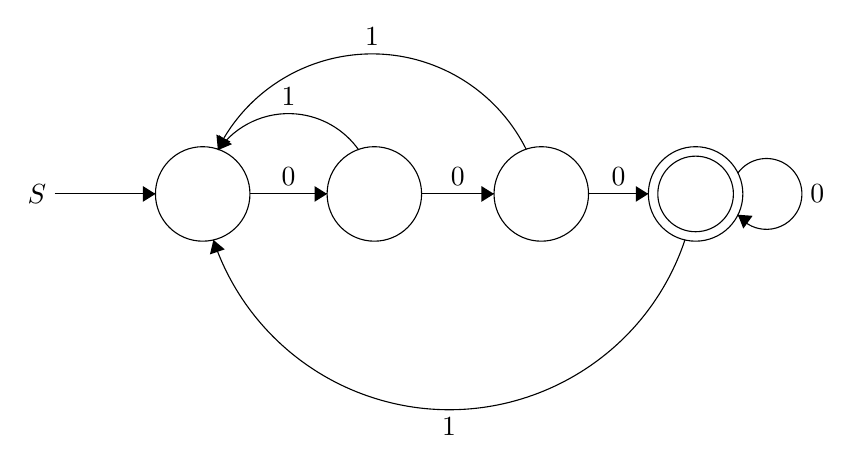
\begin{tikzpicture}[scale=0.2]
            \tikzstyle{every node}+=[inner sep=0pt]
            \draw [black] (13.8,-12.7) circle (3);
            \draw [black] (24.7,-12.7) circle (3);
            \draw [black] (35.3,-12.7) circle (3);
            \draw [black] (45.1,-12.7) circle (3);
            \draw [black] (45.1,-12.7) circle (2.4);
            \draw [black] (16.8,-12.7) -- (21.7,-12.7);
            \fill [black] (21.7,-12.7) -- (20.9,-12.2) -- (20.9,-13.2);
            \draw (19.25,-12.2) node [above] {$0$};
            \draw [black] (27.7,-12.7) -- (32.3,-12.7);
            \fill [black] (32.3,-12.7) -- (31.5,-12.2) -- (31.5,-13.2);
            \draw (30,-12.2) node [above] {$0$};
            \draw [black] (38.3,-12.7) -- (42.1,-12.7);
            \fill [black] (42.1,-12.7) -- (41.3,-12.2) -- (41.3,-13.2);
            \draw (40.2,-12.2) node [above] {$0$};
            \draw [black] (14.789,-9.908) arc (144.75241:35.24759:5.462);
            \fill [black] (14.79,-9.91) -- (15.66,-9.54) -- (14.84,-8.97);
            \draw (19.25,-7.1) node [above] {$1$};
            \draw [black] (14.757,-9.867) arc (153.48523:26.51477:10.944);
            \fill [black] (14.76,-9.87) -- (15.56,-9.37) -- (14.67,-8.93);
            \draw (24.55,-3.31) node [above] {$1$};
            \draw [black] (44.424,-15.618) arc (-18.48859:-161.51141:15.789);
            \fill [black] (14.48,-15.62) -- (14.26,-16.54) -- (15.2,-16.22);
            \draw (29.45,-26.9) node [below] {$1$};
            \draw [black] (4.4,-12.7) -- (10.8,-12.7);
            \draw (3.9,-12.7) node [left] {$S$};
            \fill [black] (10.8,-12.7) -- (10,-12.2) -- (10,-13.2);
            \draw [black] (47.78,-11.377) arc (144:-144:2.25);
            \draw (52.35,-12.7) node [right] {$0$};
            \fill [black] (47.78,-14.02) -- (48.13,-14.9) -- (48.72,-14.09);
            \end{tikzpicture}
    \end{center}
\end{example}
\begin{example}
    
    构造$M$,使得$L(M) = \set*{0x0 | x \in \set*{0,1}^*}$。 

    \begin{center}
        \begin{tikzpicture}[scale=0.2]
        \tikzstyle{every node}+=[inner sep=0pt]
        \draw [black] (26.6,-24.4) circle (3);
        \draw (26.6,-24.4) node {$\epsilon$};
        \draw [black] (15.7,-17.2) circle (3);
        \draw (15.7,-17.2) node {奇0};
        \draw [black] (37.6,-31.8) circle (3);
        \draw (37.6,-31.8) node {奇1};
        \draw [black] (37.6,-31.8) circle (2.4);
        \draw [black] (15.7,-31.8) circle (3);
        \draw (15.7,-31.8) node {偶0};
        \draw [black] (15.7,-31.8) circle (2.4);
        \draw [black] (37.6,-17.2) circle (3);
        \draw (37.6,-17.2) node {偶1};
        \draw [black] (24.1,-22.75) -- (18.2,-18.85);
        \fill [black] (18.2,-18.85) -- (18.6,-19.71) -- (19.15,-18.88);
        \draw (22.12,-20.3) node [above] {$0$};
        \draw [black] (29.09,-26.07) -- (35.11,-30.13);
        \fill [black] (35.11,-30.13) -- (34.73,-29.26) -- (34.17,-30.09);
        \draw (33.07,-27.6) node [above] {$1$};
        \draw [black] (15.7,-20.2) -- (15.7,-28.8);
        \fill [black] (15.7,-28.8) -- (16.2,-28) -- (15.2,-28);
        \draw (15.2,-24.5) node [left] {$0$};
        \draw [black] (18.7,-17.2) -- (34.6,-17.2);
        \fill [black] (34.6,-17.2) -- (33.8,-16.7) -- (33.8,-17.7);
        \draw (26.65,-16.7) node [above] {$1$};
        \draw [black] (34.6,-31.8) -- (18.7,-31.8);
        \fill [black] (18.7,-31.8) -- (19.5,-32.3) -- (19.5,-31.3);
        \draw (26.65,-32.3) node [below] {$0$};
        \draw [black] (37.6,-28.8) -- (37.6,-20.2);
        \fill [black] (37.6,-20.2) -- (37.1,-21) -- (38.1,-21);
        \draw (38.1,-24.5) node [right] {$1$};
        \end{tikzpicture}
        \end{center}
\end{example}

\begin{example}
    构造$M$,使得$L(M) = \set*{0x0 | \text{x看作二进制时,}x \mod 3 = 1}$。 
\begin{center}
    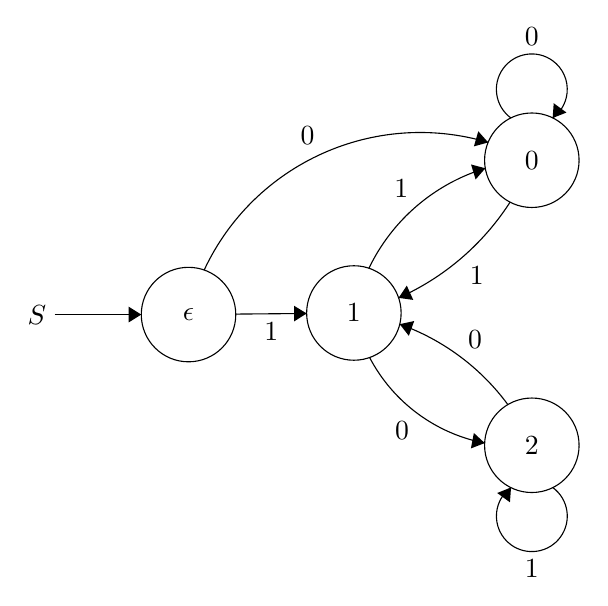
\begin{tikzpicture}[scale=0.2]
    \tikzstyle{every node}+=[inner sep=0pt]
    \draw [black] (38.9,-19.1) circle (3);
    \draw (38.9,-19.1) node {$0$};
    \draw [black] (27.6,-28.8) circle (3);
    \draw (27.6,-28.8) node {$1$};
    \draw [black] (38.9,-37.2) circle (3);
    \draw (38.9,-37.2) node {$2$};
    \draw [black] (17.1,-28.9) circle (3);
    \draw (17.1,-28.9) node {$\epsilon$};
    \draw [black] (28.553,-25.963) arc (154.34808:106.93797:12.128);
    \fill [black] (35.95,-19.61) -- (35.04,-19.37) -- (35.33,-20.32);
    \draw (30.61,-21.52) node [above] {$1$};
    \draw [black] (35.913,-37.06) arc (-100.87688:-152.3746:10.496);
    \fill [black] (35.91,-37.06) -- (35.22,-36.42) -- (35.03,-37.4);
    \draw (30.66,-35.67) node [below] {$0$};
    \draw [black] (37.52,-21.759) arc (-32.71252:-66.00143:16.293);
    \fill [black] (30.44,-27.84) -- (31.37,-27.97) -- (30.96,-27.06);
    \draw (35.4,-25.81) node [below] {$1$};
    \draw [black] (37.577,-16.42) arc (234:-54:2.25);
    \draw (38.9,-11.85) node [above] {$0$};
    \fill [black] (40.22,-16.42) -- (41.1,-16.07) -- (40.29,-15.48);
    \draw [black] (40.223,-39.88) arc (54:-234:2.25);
    \draw (38.9,-44.45) node [below] {$1$};
    \fill [black] (37.58,-39.88) -- (36.7,-40.23) -- (37.51,-40.82);
    \draw [black] (30.509,-29.512) arc (70.37322:36.37529:14.642);
    \fill [black] (30.51,-29.51) -- (31.09,-30.25) -- (31.43,-29.31);
    \draw (35.3,-31.06) node [above] {$0$};
    \draw [black] (8.6,-28.9) -- (14.1,-28.9);
    \draw (8.1,-28.9) node [left] {$S$};
    \fill [black] (14.1,-28.9) -- (13.3,-28.4) -- (13.3,-29.4);
    \draw [black] (20.1,-28.87) -- (24.6,-28.83);
    \fill [black] (24.6,-28.83) -- (23.8,-28.34) -- (23.8,-29.34);
    \draw (22.35,-29.36) node [below] {$1$};
    \draw [black] (18.093,-26.074) arc (154.9625:73.44927:15.144);
    \fill [black] (36.13,-17.97) -- (35.5,-17.26) -- (35.22,-18.22);
    \draw (24.66,-18.16) node [above] {$0$};
    \end{tikzpicture}
\end{center}
\end{example}

\end{document}
